\documentclass[12pt,a4paper,twocolumn]{article}

\usepackage[english]{babel} 		%% englische Sprache

\usepackage[latin1,applemac]{inputenc}	%% deutsche Umlaute wie normale
 					%% Buchstaben verwenden 
 					%% (ansonsten muesste � durch a getippt werden)
\usepackage{a4wide} 			%% kleinere Seitenr�nder

\usepackage{amssymb,amsthm,amsfonts, amsmath}
								%% diverse Matheerweiterungen, z.B. \implies
 								%% diverse Matheerweiterungen, z.B. \mathbb{R}
%\usepackage{stmaryrd} 			%% weitere Symbole
\usepackage{epsfig} 			%% um eps-Dateien einzubinden (\epsfig{file=...})
\usepackage{longtable} 			%% fuer Tabellen ueber mehrere Seiten
\usepackage{color}
\usepackage{hyperref}
\usepackage{dsfont}
\usepackage{caption}
\usepackage{multirow}


\title{ \textcolor{red}{\textbf{\textit{Some super concise and informative title}}} \\ Data Analysis Project for \\ \textit{Machine Learning: Basic Principles}}
%\author{H�ctor Laria Mantec�n and Maximilian Proll}
\date{\today}

\begin{document}

\maketitle

\begin{abstract}
\textit{
Precise summary of the whole report, previews the contents and results. Must be a single paragraph between 100 and 200 words.
} 

\end{abstract}

\section{Introduction}

The name Spotify will ring a bell and Spotify is probably the most famous company in the music streaming business. Within six years they turned free music into a \$10+ billion valuation with more than 50 million users, 12.5 million of which pay for their service.

How did Spotify achieve that? For one the appealing so-called freemium business model offered users a good (and legal) alternative to piracy and the pay-per-track model of iTunes. But on the other side Spotify particularly shined with state of the art product features, which include a unprecedent recommendation system for tracks, albums and playlists.

One crucial step for those above-mention recommendation systems is to understand the genre which a user seems to like. If a user listens a lot to Jazz, 


\textit{
Background, problem statement, motivation, many references, description of contents. Introduces the reader to the topic and the broad context within which your research/project fits
\begin{itemize}
\item What do you hope to learn from the project?
\item What question is being addressed?
\item Why is this task important? (motivation)
\end{itemize}
Keep it short (half to 1 page).
}

\section{Data analysis}
This competition is performed on two datasets, a training and a test dataset with $4.363$ resp. $6.544$ songs. Each dataset has a total of $264$ features, which will be used for predicting one of $10$ classes. The features con be grouped into the 3 main components of music: timbre, pitch and rhythm. The $10$ classes are:  Pop Rock, Electronic, Rap, Jazz, Latin, R\&B, International, Country, Reggae and Blues.

In order to better visualise the training data we performed the \textit{t-Distributed Stochastic Neighbor Embedding} \cite{tsne} (\textbf{t-SNE}) with $3$ remaining dimensions. The result of this award-winning embedding is shown in Figure \ref{pic:tsne}.

\begin{figure}
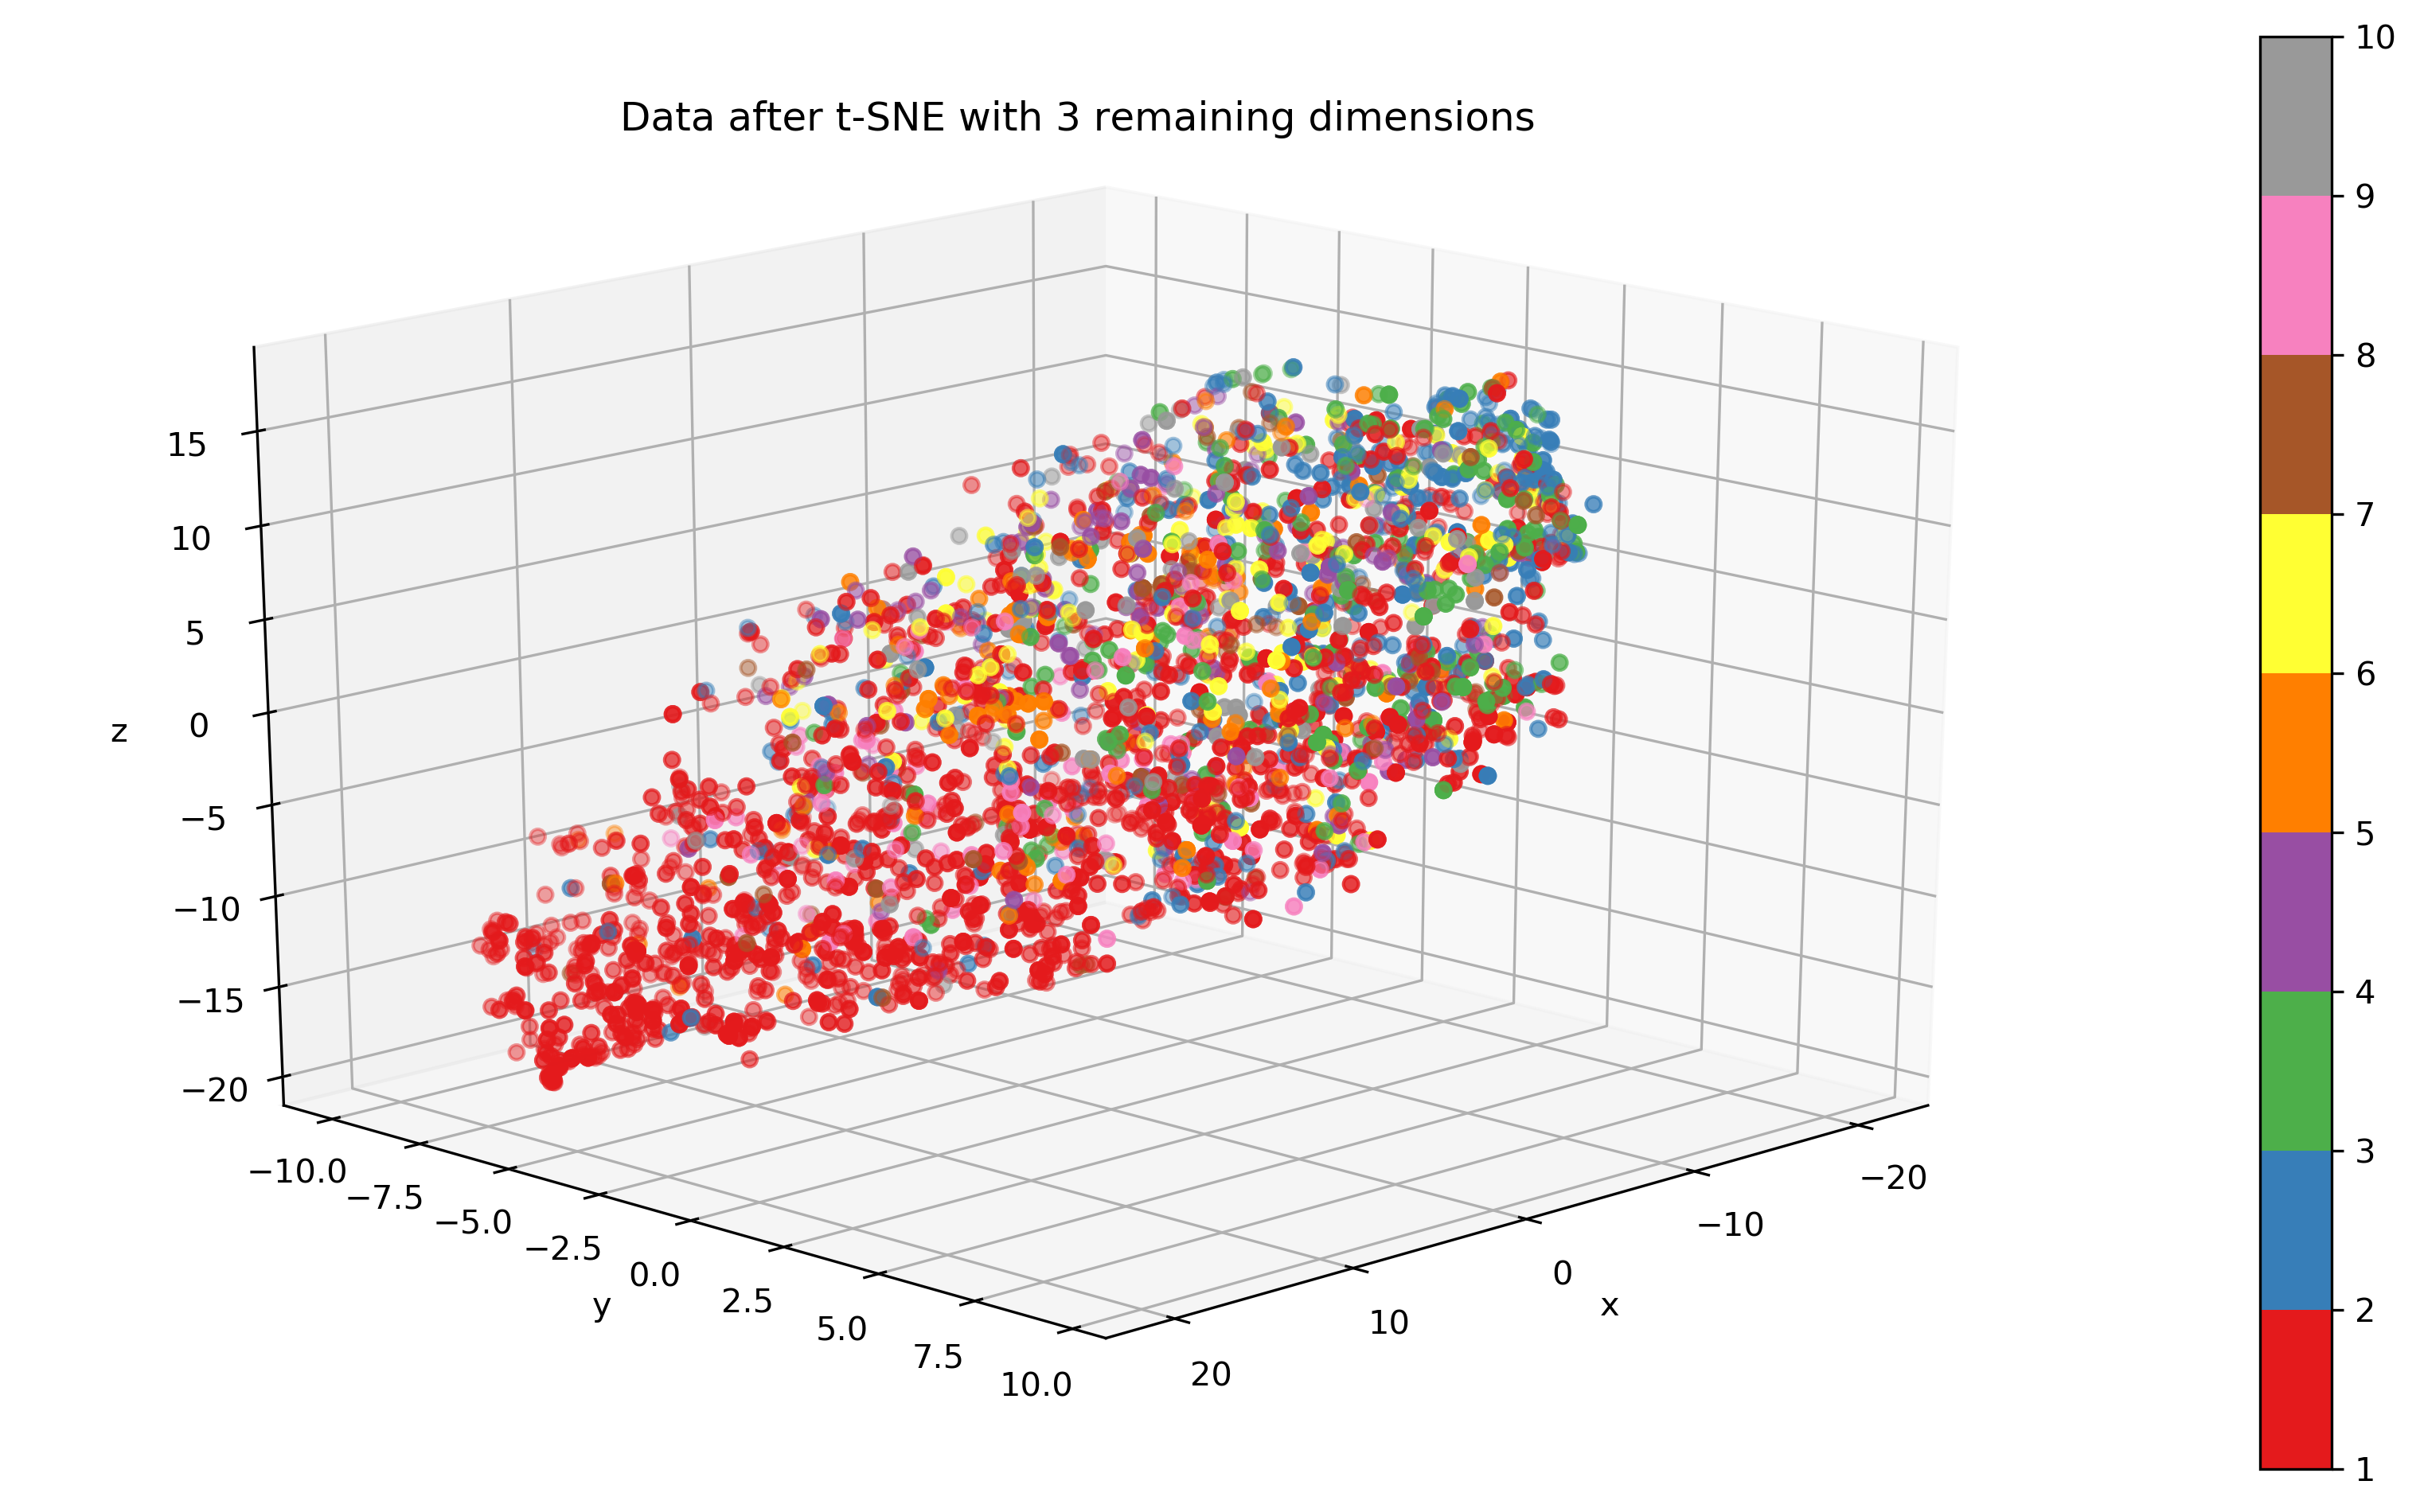
\includegraphics[width=\linewidth]{report_files/TSNE_data.png}
\caption{Data visualisation after t-SNE with $3$ dimensions}
\label{pic:tsne}
\end{figure}

This figure shows, that there does not exist a trivial separation of all 10 classes after the t-SNE in a 3-dimensional space. This might already lower somehow the expectations for the prediction accuracy. 

It is also important to know the distribution of the given training dataset. The distribution is shown in figure \ref{pic:classdistribution}.

\begin{figure}
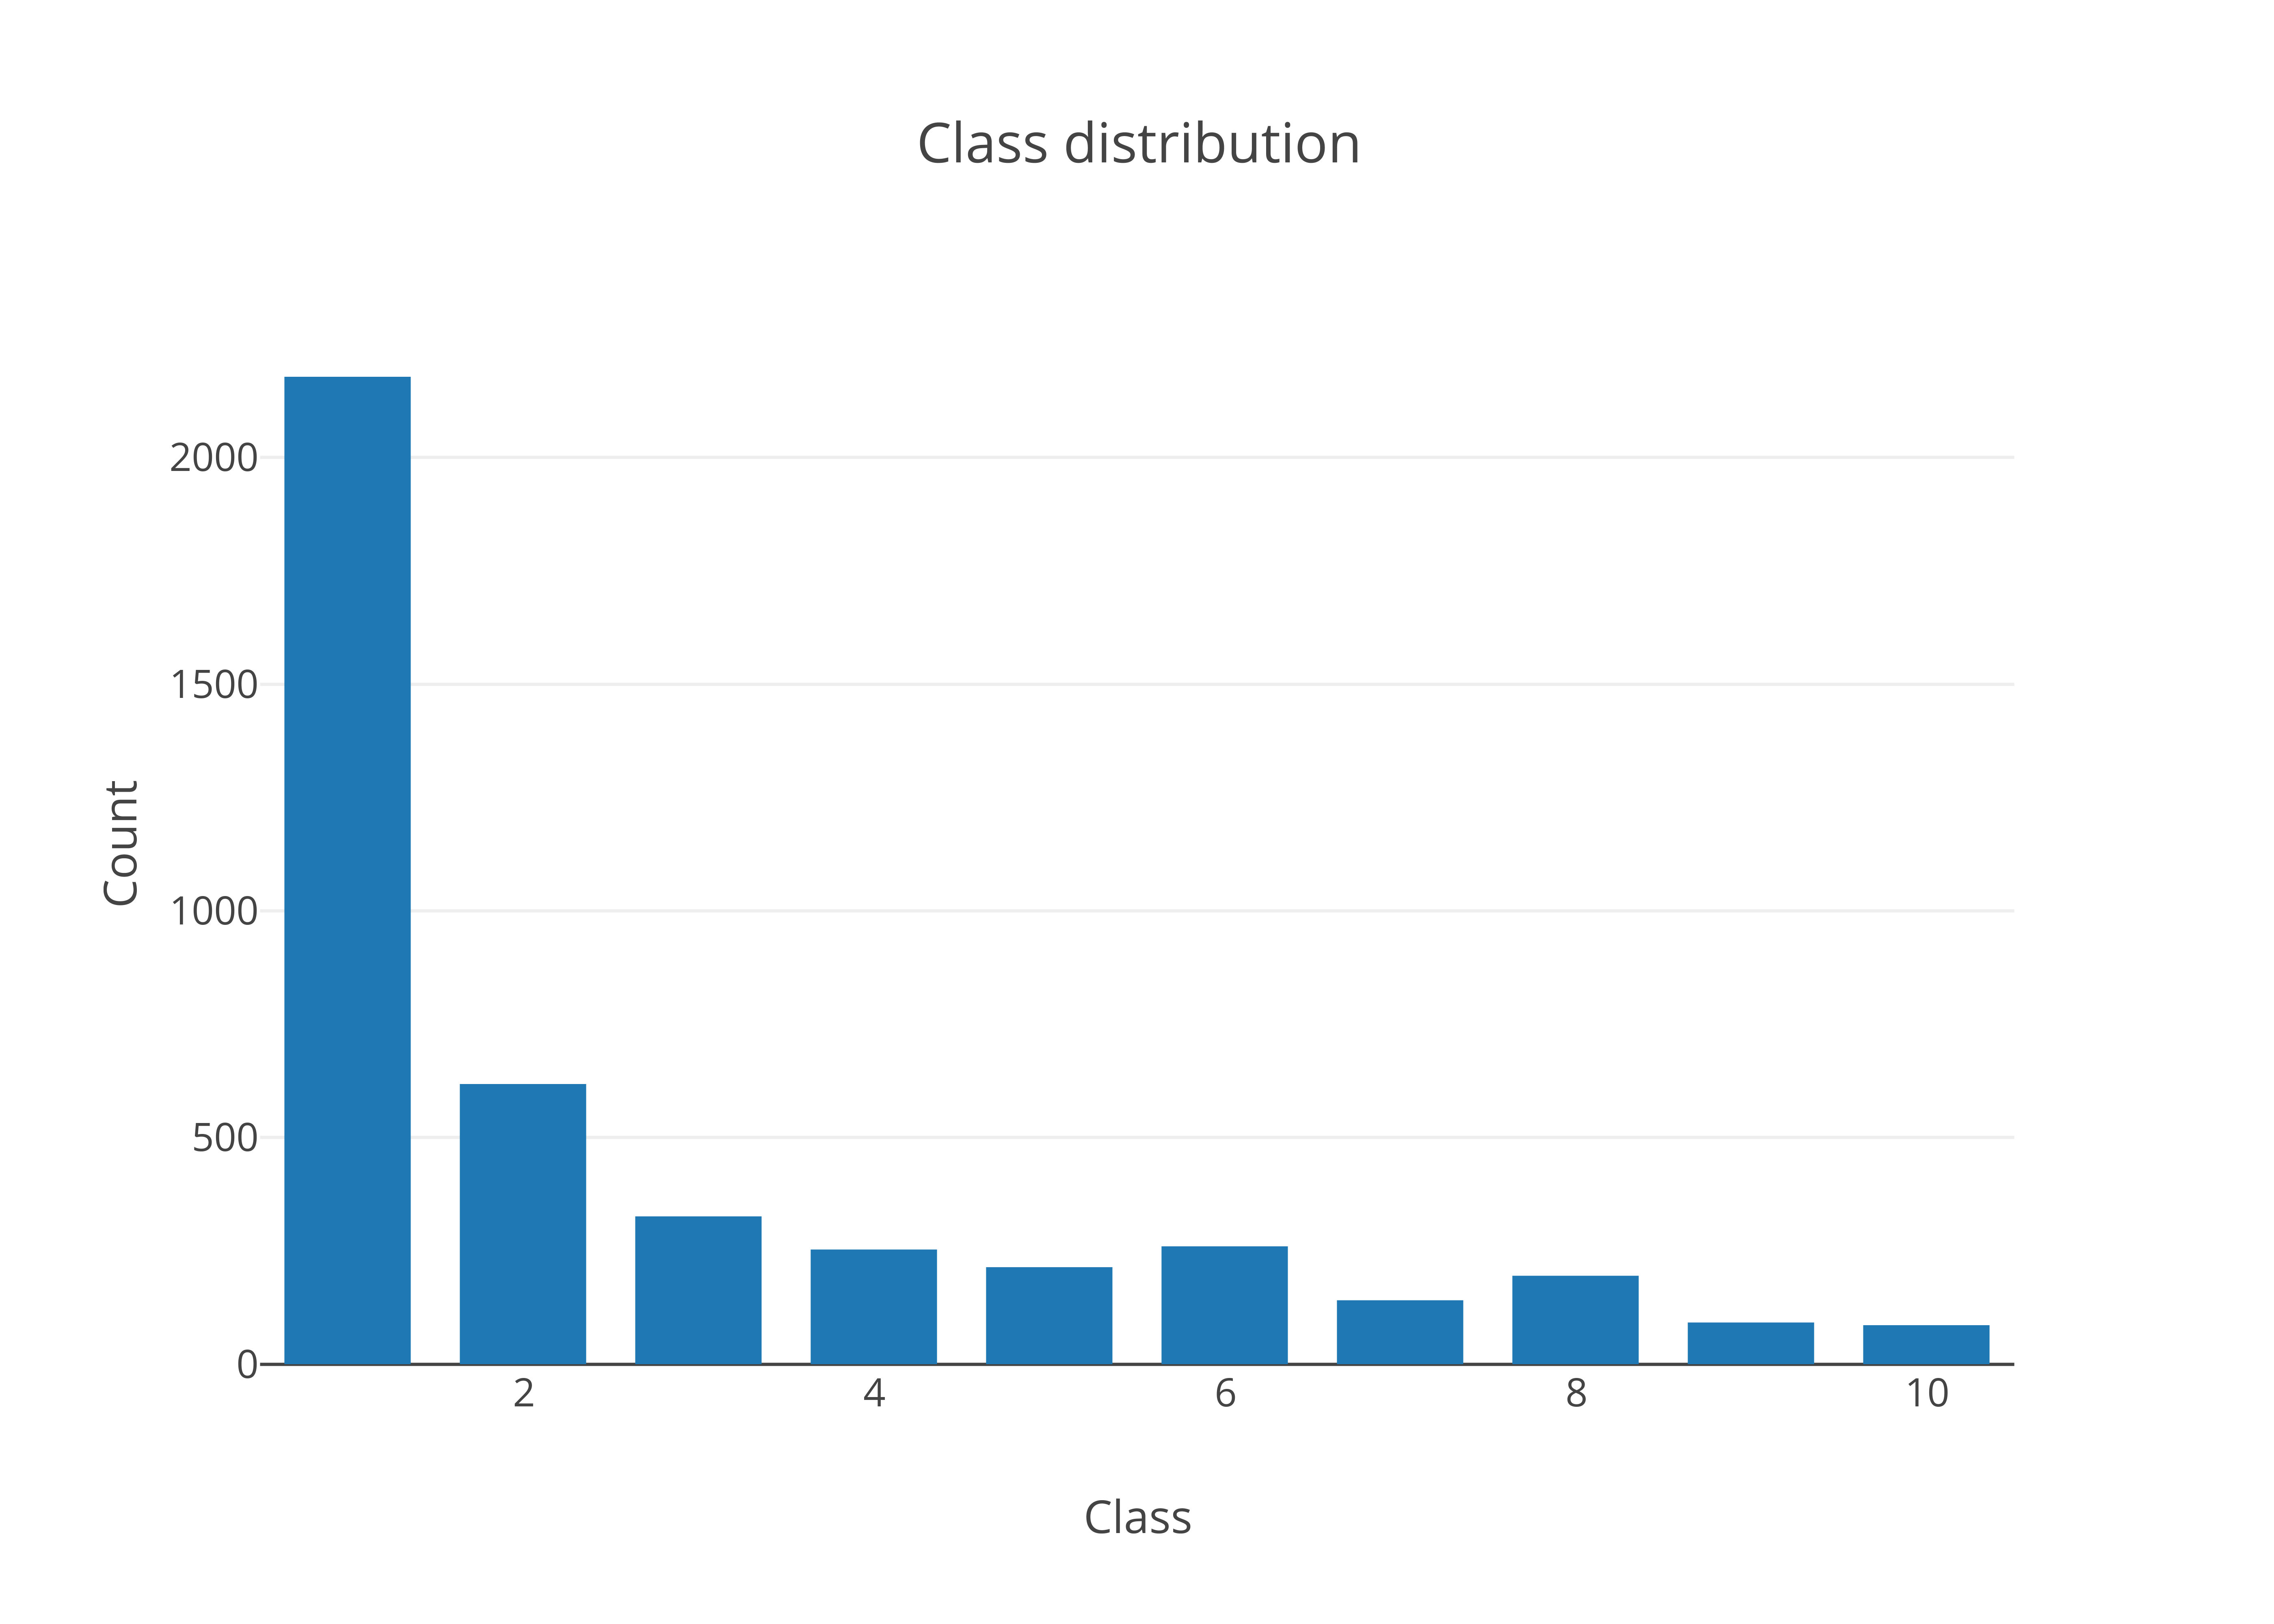
\includegraphics[width=\linewidth]{report_files/Class_distribution.png}
\caption{Class distribution}
\label{pic:classdistribution}
\end{figure}

This distribution shows very clearly that the training data is skewed, which means that the predictor will be able to generalise better for the majority classes and worse for those classes that have not many samples representing them.

%in case we need to fill more space we could add a boxplot of the 264 features.

%\textit{
%Briefly describe data (class distribution, dimensionality) and how will it affect classification. Visualize the data. Don�t focus too much on the meaning of the features, unless you want to.
%\begin{itemize}
%\item Include histograms showing class distribution.
%\end{itemize}
%}

\section{Methods and experiments}
\subsection{Overall approach}

To achieve best overall results we tried various machine learning techniques ranging from logistic regression (LogReg) and support vector machines (SVM) to na�ve Bayes classifiers (NB) and neural networks (NN). Common for all machine learning techniques was, that we first standardised the training as well as the test data prior to performing any analysis. This step is crucial as it helps to reduce multicollinearity within the data and helps to improve the generalisation. This behaviour is backed up by comparing the accuracy of the prediction of the training data without standardisation ($p$) and with standardisation ($p_{st}$), which is summarised in table \ref{tab:accuracystandard}.

\begin{table}
\centering
\begin{tabular}{c|c|c}
ML technique & $p$ & $p_{st}$ \\ \hline
LogReg & 0.66 & 0.74 \\
SVM & 0.03 & 0.22 \\
NB & 0.46 & 0.52 \\
NN & 0.55 & 0.73
\end{tabular}
\caption{Comparison of accuracy of training data without standardisation and with  standardisation}
\label{tab:accuracystandard}
\end{table}

In order to prevent our analysis against heavy overfitting we chose to implement cross-validation for all machine learning techniques. We associated randomly 20\% of the training set to be the validation set. We then trained the model with the remaining 80\% of the training set and validating the analysis on the validation set. This is done multiple times and averaged.

\subsection{Logistic Regression}
We first approached the considered for this set up was Logistic Regression and discarded Linear Regression, as it is obvious the data is highly non-linear. We changed fist the penalty, using L1 regularisation in favour of L2, delivering better results.

We also tweaked the stopping criteria to get the best performance with the less time expenditure. For the solver, we trained with liblinear and saga, which are recommended for large datasets, and newton-cg and lbfgs, recommended for multiclass problems. The changes delivered minimal to no advantage on the accuracy.

We used the warm start technique for every solver, without luck either.

\subsection{Support Vector Machines}
SVMs were trained with several kernels, and its accuracy was close to Logistic Regression. Although they were easily overfitted. Penalty parameter $C$ was set to $0.8$. All trainings were performed with balanced class weight, which uses the values of the labels to automatically adjust weights inversely proportional to class frequencies in the input data. As a measure of dealing with skewed classes.

We made use of a linear kernel, a polynomial, RBF and a sigmoid. Linear and RBF validation error was good, but they performed bad on the test set. Polynomial was overfitting with ease, and sigmoid wasn't complex enough to beat the benchmark.

\subsection{Na�ve Bayes}
Here we tried two different Na�ve algorithms, Gaussian Na�ve Bayes and Multinomial Na�ve Bayes. The performance for both of them though wasn't acceptable as none beat the benchmark.

Gaussian Na�ve Bayes was set up with no prior and a smoothing parameter of 1. One aspect worth noting is that this algorithm needs data samples $<0$, therefore we had to rescale the data in the range of $[0,1]$ instead.

Multinomial Na�ve Bayes was scaled normally, and didn't use any prior either.

\subsection{Neural Networks}
For this approach, we tried a fixed architecture of 5 fully connected hidden layers with 120 to 250 neurons per layer. We tested several different settings for the hyper-parameters such as the activation function, the update technique and the constancy as well as the initialisation value of the learning rate.

For the activation function we variated between the logistic sigmoid function, the the hyperbolic tangent function and the rectified linear unit function.

Apart from the simple stochastic gradient descent we tried also an optimiser from the family of quasi-Newton methods and the well known update technique Adam \cite{DBLP:journals/corr/KingmaB14}, a stochastic gradient-based optimiser.

Finally we used three different learning rate schedules for weight updates. The most commonly used is a constant learning rate, but we also used a gradually decreasing learning rate each time step $t$ using an inverse scaling  and finally an adaptive learning rate, which keeps the learning rate constant as long as training loss keeps decreasing and each time two consecutive epochs fail to decrease training loss or fail to increase validation score, the current learning rate is divided by 5.

The initialisation value of the learning rate was decreased if no convergence occurred within a reasonable number of iterations.

\textit{
Explain your whole approach (you can include a block diagram showing the steps in your process).
\begin{itemize}
\item What methods/algorithms, why were the methods chosen.
\item What evaluation methodology (cross CV, etc.).
\end{itemize}
}

\section{Results}

\textit{
Summarize the results of the experiments without discussing their implications.
\begin{itemize}
\item Include both performance measures (accuracy and LogLoss).
\item How does it perform on kaggle compared to the train data.
\item Include a confusion matrix.
\end{itemize}
}

We can see measurements of the methods chosen in Table~\ref{table:measurements}.

\begin{table}[h]
\centering
\caption{Performance measurements (accuracy and LogLoss), and performance on Kaggle competition.}
\label{table:measurements}
\begin{tabular}{llcc}
                                  &         & \textbf{Validation} & \textbf{Kaggle} \\ \hline
\multirow{2}{*}{\textbf{Log Reg}} & Accuracy  & 0.74329             & 0.65021         \\ \cline{2-2}
                                  & Log. Loss & -                   & 0.17736         \\ \hline
\multirow{2}{*}{\textbf{SVM}}     & Accuracy  & 0.85835             & 0.60238         \\ \cline{2-2}
                                  & Log. Loss & -                   & 0.25370         \\ \hline
\multirow{2}{*}{\textbf{NB}}      & Accuracy  & -                   & 0.61720         \\ \cline{2-2}
                                  & Log. Loss & -                   & 0.19949         \\ \hline
\multirow{2}{*}{\textbf{NN}}      & Accuracy  & 0.73779             & 0.63523         \\ \cline{2-2}
                                  & Log. Loss & -                   & 0.19893         \\ \hline
\end{tabular}
\end{table}

\section{Discussion/Conclusions}

\textit{
Interpret and explain your results
\begin{itemize}
\item Discuss the relevance of the performance measures (accuracy and LogLoss) for
imbalanced multiclass datasets.
\item How the results relate to the literature.
\item Suggestions for future research/improvement.
\item Did the study answer your questions?
\end{itemize}
}

%\textit{List of all the references cited in the document
%}
\bibliography{bibliography}{}
\bibliographystyle{alpha}

\section*{Appendices}

\textit{Additional information that is not essential to explain your findings, but supports your work. For example, source code, additional images, mathematical derivations, etc. \\
If you include source code, don�t include the whole code, focus only on the most important parts, for example, a function implementing a specific algorithm
}


\end{document}
